\documentclass[12pt, a4paper,brazil,oneside]{article}
\usepackage[bottom=2cm,top=3cm,left=3cm,right=2cm]{geometry}
\usepackage{xcolor}
\usepackage{fancyhdr}
\usepackage[utf8]{inputenc}
\usepackage{lscape}
\usepackage{setspace}
\usepackage[brazil]{babel}
\usepackage{setspace}
\usepackage{indentfirst}
\usepackage{amsmath}
\usepackage{adjustbox}
\usepackage{placeins}
\usepackage{graphicx}
\usepackage{url} 
\usepackage{enumerate} 
\usepackage{amsmath,amsthm,amsfonts,amssymb,amsxtra}
\usepackage{bm} 
\usepackage[alf,bibjustif]{abntex2cite}
\usepackage{amsthm}
\newtheorem{deff}{Definição}
\newtheorem{teo}{Teorema}
\usepackage{multirow}
\usepackage{float}
\usepackage{tabularx}
\usepackage{subfig}

\renewcommand{\baselinestretch}{1.2}

\begin{document}
	
	%CAPA
	\onehalfspacing
	\thispagestyle{empty}
	\begin{center}
		\large\singlespacing{\textbf{UNIVERSIDADE FEDERAL DE ALFENAS \\
				UNIFAL}}\\
		\textbf{Programa de Pós-Graduação em Estatística Aplicada e Biometria}\\	
		
		\vspace{4cm}
		\textbf{WALEF MACHADO DE MENDONÇA}\\
		\vspace{6cm}
		\textbf{O seguro rural no Brasil: uma análise de agrupamento considerando a localização espacial}\\
		\vspace{9cm}
		\textbf{Alfenas/MG\\
			2020}
	\end{center}
	%==============================================
	%PROJETO
	\newpage \thispagestyle{empty}
	\begin{center}
		\textbf{WALEF MACHADO DE MENDONÇA}
		\vspace{5cm}\\
		\textbf{O seguro rural no Brasil: uma análise de agrupamento considerando a localização espacial}\\
		\begin{flushright}
			\begin{minipage}{10cm}
				\begin{quote}
					\vspace{3cm}
					Projeto de dissertação apresentado ao Programa de Pós Graduação em Estatística Aplicada e Biometria da Universidade Federal de Alfenas - UNIFAL/MG. \\
					Orientadora: Profa. Dra. Patrícia de Siqueira Ramos. \\
				\end{quote}
			\end{minipage}
		\end{flushright}
		\vspace{8cm}
		Alfenas/MG\\2020
	\end{center}
	
	%==============================================
	%LISTA DE TABELAS
	\newpage
	\listoftables
	%==============================================
	%LISTA DE FIGURAS
	\newpage
	\listoffigures
	%==============================================
	%SUMARIO
	\newpage
	\tableofcontents
	%==============================================
	%INTRODUÇÃO
	\newpage
	\section{Introdução}
	
	O ambiente no qual se desenvolvem as atividades agropecuárias apresenta elevado risco e significativa incerteza. Essa insegurança se deve, principalmente, às instabilidades climáticas e ameaças sanitárias, que podem afetar a produção, ou à razões de mercado, como variações das taxas de câmbio e juros, ou a condições ligadas ao ambiente de negócios, tais como alterações em marcos regulatórios e em políticas públicas Todas essas variáveis, relacionadas aos mercados agropecuários, geram variações na renda do setor, que são comumente enfrentadas por meio de políticas de apoio à gestão de riscos. 

	% Tipos de risco (tem um artigo que trata os tipos e formas de mitigação)
	
	O gerenciamento de riscos agropecuários pode ocorrer de diversas maneiras, no entanto, a contratação de seguro rural é uma das formas mais usuais. Essa modalidade de seguro atua no sentido de amenizar as perdas e possibilitar a recuperação da capacidade financeira do produtor na ocorrência de sinistros. O seguro rural propicia um ambiente mais favorável ao desenvolvimento das atividades agropecuárias pois proporciona a garantia do fluxo de renda, favorece um aumento da área plantada e facilita a obtenção de financiamento. Além disso, se mostra um instrumento que possibilita o compartilhamento do risco da agropecuária com outros agentes e setores econômicos. 
	
	É importante destacar que o mercado de seguro rural não se consolida sem a participação do Estado. Destacam-se problemas como os elevados investimentos e custos administrativos, a possibilidade de riscos catastróficos, a forte influência do risco moral e da seleção adversa na formação das carteiras, como fatores que limitam a eficiência da iniciativa privada na oferta de produtos. Nesse sentido, o poder público é demandado a interferir no mercado, seja atuando diretamente como seguradora, seja criando programas que estimulem a oferta e a demanda por produtos de seguro.
	
	Como mecanismo de estímulo para o desenvolvimento do seguro rural, o governo brasileiro criou o Programa de Subvenção ao Prêmio do Seguro Rural (PSR), instituído pela Lei 10.823/2003 e decreto nº 5.121/2004 (BRASIL, 2018). Tal política do governo busca tornar o seguro rural mais acessível aos produtores, dividindo os custos de aquisição da apólice entre o governo e os produtores. 
	
	
	\newpage
	\section{Objetivos}\label{objetivos}
	
	O objetivo desse trabalho é identificar grupos de municípios com características semelhantes em relação à adesão ao seguro rural em 2018 através do agrupamento de dados multivariados e suas distribuições espaciais. De forma que os agrupamentos obtidos levem em consideração não apenas o valor das variáveis de seguro rural mas também seu posicionamento geográfico. 
	
	\subsection{Objetivos Específicos}
	
	\begin{itemize}
		\item Apresentar um procedimento para o agrupamento com base na distribuição espacial de dados multivariados.
		
		\item Subsidiar a tomada de decisões sobre políticas públicas de estímulo à demanda por produtos de seguro específicas para cada grupo de municípios.
	\end{itemize} 	
	
	\newpage
	\section{Referencial Teórico}\label{referencial}
	
	\subsection{Seguro rural}
	% Importância do setor agropecuario 
	% Risco do setor 
	% Mecanismos de mitigação de riscos 
	% Zarc como	instrumento de apoio às	ações de política agrícola (Aqui?)
		
	\subsubsection{O seguro rural no Brasil}
	% Seguro rural
	% Problemas no funcionamento de mercado puro 
	% Ações pra mitigar risco Souza (2000)
	% Necessidade de atuação pública (MACEDO, 2013)
	
	\subsubsection{O Programa de Subvenção ao Prêmio do Seguro Rural}		
	% Antecedentes (?)
	% Características do Programa
	% Evolução do PSR 
		% Número de produtores
		% Número de apólices
		% Subvenção
		% Área segurada
		% Capital 
		% Participação nas subvenções por regiões (?)

	\subsection{Análise Multivariada}
	

	
	Em uma pesquisa, os dados obtidos são considerados multivariados quando cada unidade amostral possui diversas variáveis aleatórias. A análise multivariada se caracteriza por um conjunto de métodos estatísticos que são utilizados para analisar as variáveis como um todo, levando-se em conta, por exemplo, a sua estrutura de correlação. Os métodos de análise multivariada possibilitam a realização de  uma avaliação muito mais ampla do conjunto de dados, permitindo encontrar padrões que, possivelmente, não seriam revelados ao se analisar cada variável separadamente (MINGOTI, 2005). 
	
	Segundo Hair et al (2009), os métodos multivariados podem ser divididos como métodos de dependência e interdependência. Se estudo envolver variáveis com uma estrutura de dependência previamente identificada aconselha-se que se faça uso de técnicas de dependência, tais como regressão múltipla, regressão logística ou análise discriminante. 
	Entretanto, se não haver uma distinção preliminar entre quais variáveis são dependentes e independentes, aconselha-se que o uso de técnicas de interdependência como análise fatorial e análise de agrupamento.
	
	
	A representação de dados multivariados se dá através de matrizes. Uma amostra aleatória que contenha $n$ unidades amostrais ou observações contendo valores de $p$ variáveis observadas dá origem a uma matriz de dados $\boldsymbol{X}$ com dimensão $n$ (linhas) por $p$ (colunas):
	
	\begin{align}\label{X}
	\boldsymbol{X}_{n \times p} =
	\left[
	\begin{array}{cccc}
	X_{11} & X_{12} & \dots & X_{1p} \\
	X_{21} & X_{22} & \dots & X_{2p} \\
	\vdots & \vdots & \ddots & \vdots \\
	X_{n1} & X_{n2} & \dots & X_{np}\\
	\end{array}
	\right],
	\end{align}
	
	\noindent em que cada unidade amostral é representada por uma linha da matriz de dados $\boldsymbol{X}$, sendo um vetor com $p$ elementos (variáveis), e cada variável é representada por uma coluna de $\boldsymbol{X}$, sendo um vetor com $n$ elementos, as observações (EVERITT; HOTHORN, 2011).
	
	A representação de dados multivariados em uma matriz como apresentada na forma da definição (\ref{X}) pode não pode não ser muito informativa, principalmente se o tamanho amostral $n$ for grande e houver um número abundante de variáveis $p$. Desse modo, torna-se relevante a utilização de medidas resumo dos dados amostrais, calculando-se a média, mediana, desvio padrão etc. de forma a sintetizar as informações dos dados da amostra (FERREIRA, 2011).  
	
	A média amostral, muito utilizada como uma medida de tendência central, torna-se o vetor de médias amostral no caso multivariado de dimensão $p \times 1$, onde cada elemento $\bar{X}_{i}$, com $i = 1,2,\cdots,p $, é a média de uma variável:
	
	\begin{align*}
	\boldsymbol{\bar{X}} = \left[
	\begin{array}{c}
	\bar{X}_1\\
	\bar{X}_2\\
	\vdots\\
	\bar{X}_p\\
	\end{array}
	\right].
	\end{align*}
	
	Como medida de dispersão dos dados, no caso multivariado, utiliza-se, no lugar da variância amostral, a matriz de covariâncias amostral $\boldsymbol{S}$ de dimensão $p \times p$. Em sua diagonal principal estão as variâncias de cada uma das $p$ variáveis, enquanto os elementos fora da diagonal principal são as covariâncias entre as variáveis. A matriz de covariâncias amostral é simétrica, ou seja,  $S_{ij}$ $=$ $S_{ji}$.
	
	
	\begin{align*}
	\boldsymbol{S} =
	\left[
	\begin{array}{cccc}
	S_{11} & S_{12} & \dots & S_{1p} \\
	S_{21} & S_{22} & \dots & S_{2p} \\
	\vdots & \vdots & \ddots & \vdots \\
	S_{p1} & S_{p2} & \dots & S_{pp} \\
	\end{array}
	\right].
	\end{align*}        
	
	A correlação também pode ser usada como uma medida de associação entre duas variáveis. Os valores do coeficiente de correlação variam entre $-1$ e $1$. Valores próximos de $1$ indicam que as variáveis estão fortemente correlacionadas de forma positiva, ou seja, grandes valores de uma estão associados a grandes valores da outra. Já valores próximos de $-1$ indicam que as variáveis estão fortemente correlacionadas de forma negativa, o que indica que grandes valores de uma estão associados a pequenos valores da outra. A matriz de correlações amostral é dada por 
	
	\begin{align*}
	\boldsymbol{R} =
	\left[
	\begin{array}{cccc}
	1      & r_{12} & \dots  & r_{1p} \\
	r_{21} & 1 & \dots  & r_{2p} \\
	\vdots & \vdots & \ddots & \vdots \\
	r_{p1} & r_{p2} & \dots  & 1\\
	\end{array}
	\right].
	\end{align*}        
	
	\noindent em que $r_{ij} = \frac{S_{ij}}{\sqrt{S_{ii} S_{jj}}}$ (FERREIRA, 2011).  
	
	\vspace{0.15cm} % só pra dar um espacinho :)
	
	Outras estatísticas descritivas, como a matriz de somas de quadrados e produtos e a matriz de correlações, podem ser consideradas, dependendo do objetivo do estudo (FERREIRA, 2011).
	
	Assim como ocorre na análise univariada, as técnicas de estatística multivariada podem ser divididas em dois grupos, as técnicas exploratórias e as técnicas de inferência estatística. O primeiro grupo constitui-se de técnicas que não dependem do conhecimento da forma matemática da distribuição de probabilidade que gerou os dados amostrais. Além disso, o uso dessas técnicas permite a identificação de padrões em dados multivariados, fazendo com que possuam grande apelo prático. São exemplos de técnicas exploratórias análise de componentes principais, análise fatorial exploratória, análise de agrupamento. Por outro lado, o grupo de técnicas de de inferência estatística têm como objetivo a estimação  parâmetros, testes de hipóteses, análise de regressão multivariada etc.  Portanto, as técnicas de inferência fazem uso da amostra para realizar inferências sobre a população de onde essa amostra foi extraída (MINGOTI, 2005).
	
	
	\subsubsection{Análise de componentes principais} \label{ACP} 
	
	A análise de componentes principais (ACP) tem como objetivo a explicação da estrutura de covariâncias das $p$ variáveis, $\boldsymbol{X}^T = [X_1 \quad X_2 \quad \dots \quad X_p]$, através de combinações lineares das variáveis originais. Os componentes principais são as $p$ combinações lineares obtidas, $\boldsymbol{Y}^T = [Y_1 \quad Y_2 \quad \dots \quad Y_p]$, e não são correlacionados entre si. Os componentes principais são ordenados de forma que suas primeiras combinações lineares já contabilizem a maior parte da variância presente em todas as variáveis originais, consequentemente, podem ser usados para fornecer uma redução das dimensões dos dados (MINGOTI, 2005; EVERITT; HOTHORN, 2011).
	
	Vários critérios podem ser adotados para selecionar o numero de componentes de forma que grande parte da variância total seja explicada por um pequeno conjunto das novas variáveis. Com um valor de k pequeno e uma grande quantidade de variação das variáveis originais explicada pelos componentes principais, ocorre uma simplificação da estrutura de covariâncias das variáveis originais. A ACP pode então ser utilizada como uma ferramenta para auxiliar em outras técnicas, como ocorre em problemas de multicolinearidade na regressão linear, por exemplo (FERREIRA, 2011).
	
	O primeiro componente principal $Y_1$ é a combinação linear
	\begin{align*}
	Y_1 = a_{11}X_1 + a_{12}X_2 + \dots + a_{1p}X_p,
	\end{align*}
	cuja variância amostral é a maior dentre todas as outras combinações lineares. O vetor de coeficientes referente ao $j$-ésimo CP é representado por $\boldsymbol{a}_j= [a_{j1} \quad a_{j2} \quad \dots \quad a_{jp}]$. É importante usar uma restrição nos valores desses coeficientes, geralmente $\boldsymbol{a}_1^T\boldsymbol{a}_1 = 1$, ou seja, a soma dos quadrados desses valores deve ser igual a $1$. Isso deve ser feito porque a variância de $Y_1$ poderia crescer de forma ilimitada apenas aumentando os coeficientes $\boldsymbol{a}_1$. A variância amostral de $Y_1$ é dada por $\boldsymbol{a}_1^T\boldsymbol{S}\boldsymbol{a}_1$, sendo $\boldsymbol{S}$ a matriz de covariâncias amostral das $X$ variáveis e $\boldsymbol{a}_1$ é o autovetor da matriz $\boldsymbol{S}$ associado ao maior autovetor $\lambda$ dessa matriz (EVERITT; HOTHORN, 2011). A obtenção de autovalores $\lambda$ e autovetores $\boldsymbol{e}$ de uma matriz quadrada $p \times p$ são tais que $\boldsymbol{A}\boldsymbol{e} = \lambda\boldsymbol{e}$. Para maiores detalhes, consultar, por exemplo, (FERREIRA, 2011).
	
	Ainda de acordo com os autores, o segundo componente principal, $Y_2$ definido como a combinação linear
	\begin{align*}
	Y_2 = a_{21}X_1 + a_{22}X_2 + \dots + a_{2p}X_p,
	\end{align*}
	ou seja, $Y_2 = \boldsymbol{a}_2^T\boldsymbol{X}$, em que $\boldsymbol{a}_2^T = [a_{21} \quad a_{22} \quad \dots \quad a_{2p}]$ e $\boldsymbol{X}^T = [X_{1} \quad X_{2} \quad \dots \quad X_{p}]$, que possui a maior variância sujeito às condições
	\begin{align*}
	\boldsymbol{a}_2^T\boldsymbol{a}_2 = 1,\\
	\boldsymbol{a}_2^T\boldsymbol{a}_1 = 0,
	\end{align*}
	em que a segunda condição garante que $Y_1$ e $Y_2$ são não correlacionados. Todos os componentes são obtidos de forma similar.
	
	O vetor de coeficientes que define o $j$-ésimo componente principal, $\boldsymbol{a}_j$ é o autovetor de $\boldsymbol{S}$ associado com o seu $j$-ésimo maior autovetor. A variância do $j$-ésimo componente principal é dada por $\lambda_j$, sendo os $\lambda_1, \lambda_2, \dots, \lambda_p$ os autovalores de $\boldsymbol{S}$ sujeitos à restrição $\boldsymbol{a}_j^T\boldsymbol{a}_j = 1$ (EVERITT; HOTHORN, 2011).
	
	A proporção da variância total de $\boldsymbol{X}$ explicada pelo $j$-ésimo componente principal é definida por
	\begin{align*}
	\dfrac{Var(Y_j)}{\textrm{Variância total de } X} = \dfrac{\lambda_j}{\textrm{traço}(\boldsymbol{S})} = \dfrac{\lambda_j}{\displaystyle\sum_{i=1}^{p}\lambda_i}.
	\end{align*}
	
	Além disso, as variâncias total e generalizada de $\boldsymbol{X}$ podem ser descritas pelas variâncias total e generalizada de $\boldsymbol{Y}$:
	\begin{align*}
	\textrm{traço}(\boldsymbol{S}) = \displaystyle\sum_{i=1}^{p}\lambda_i = S_1^2 + S_2^2 + \dots + S_p^2 \quad \textrm{ e} \quad |\boldsymbol{S}| = \prod_{i=1}^{p}\lambda_i.
	\end{align*}
	
	Dessa forma, os vetores $\boldsymbol{X}$ e $\boldsymbol{Y}$ são equivalentes em relação a essas duas medidas de variação. Além disso, sempre o primeiro componente principal tem a maior proporção de explicação da variância total de $\boldsymbol{X}$ (MINGOTI, 2005).
	
	De acordo com Everitt e Hothorn (2011), os primeiros $k$ componentes, em que $k < p$, explicam uma proporção da variância total,
	\begin{align*}
	\dfrac{\displaystyle\sum_{j=1}^{k}Var(Y_j)}{\textrm{Variância total de } X} = \dfrac{\displaystyle\sum_{j=1}^{k}\lambda_j}{\textrm{traço}(\boldsymbol{S})} = \dfrac{\displaystyle\sum_{j=1}^{k}\lambda_j}{\displaystyle\sum_{j=1}^{p}\lambda_j}.
	\end{align*}
	
	Os componentes principais podem ser obtidos a partir da matriz de covariâncias amostrais $\boldsymbol{S}$ ou a partir da matriz de correlações amostrais $\boldsymbol{R}$. Extrair os componentes da matriz de covariâncias deve ser preferido quando as variáveis originais estão na mesma escala, o que é raro ocorrer. Extrair os componentes como os autovetores de $\boldsymbol{R}$ é equivalente a calcular os componentes das variáveis originais para depois padronizar cada um para ter variância igual a $1$ (EVERITT; HOTHORN, 2011).
	
	Ainda segundo Everitt e Hothorn (2011), os componentes principais são variáveis aleatórias que podem ser observadas apenas a partir da observação de um vetor aleatório $\boldsymbol{X}$. Os escores dos \textit{CPs} são obtidos pela substituição dos valores observados de $\boldsymbol{X}$ em cada um dos componentes $Y_j$. Se os \textit{CPs} forem obtidos a partir da matriz de covariâncias $\boldsymbol{S}$, os escores $Y^*_{ji}$ dos $k$ componentes para cada observação $i$ são dados por:  
	
	\begin{align*}
	Y^*_{1i} & =\boldsymbol{a}_1^T\boldsymbol{X}_i\\
	Y^*_{2i} & =\boldsymbol{a}_2^T\boldsymbol{X}_i\\
	&\vdots\\
	Y^*_{ki} & =\boldsymbol{a}_k^T\boldsymbol{X}_i.
	\end{align*}
	
	Estes são geralmente utilizados na condução de análises estatísticas de dados ou simplesmente para ordenação, identificando aquelas observações que possuem os maiores ou menores valores globais dos componentes (MINGOTI, 2005).
	
	\subsubsection{Análise de agrupamento} 
	
	A análise de agrupamento, também conhecida como classificação, \textit{cluster analysis} ou \textit{unsupervised learning}, é uma técnicas exploratórias que tem como objetivo encontrar partições (ou grupos) dos elementos de uma amostra de forma que as observações de um mesmo grupo sejam similares entre si em relação às variáveis medidas e que as observações de grupos diferentes sejam heterogêneas em relação a essas mesmas variáveis (MINGOTI, 2005).
	
	O termo ``análise de agrupamento'' é uma expressão genérica que inclui vários métodos numéricos que têm como objetivo encontrar grupos de observações homogêneas. Esses métodos buscam dar uma formalização para o que os seres humanos conseguem fazer eficiente em duas ou três dimensões, por exemplo, por meio de diagramas de dispersão. Na análise de agrupamento, grupos são identificados pela avaliação das distâncias entre os pontos (EVERITT; HOTHORN, 2011).
	
	
	A título de ilustração, considere um conjunto de dados simulados em que há $n=300$ observações e duas variáveis aleatórias contínuas $p=2$. O objetivo é agrupar os dados em relação às duas variáveis. O diagrama de dispersão obtido se encontra no Gráfico \ref{fake_cluster} e é possível identificar $4$ agrupamentos, apenas pela análise visual. Se houvesse mais uma variável e, consequentemente mais uma dimensão, ainda seria possível imaginar um gráfico com os pontos. Porém, com mais de três dimensões a visualização dos dados torna-se mais complexa (BARTHOLOMEW et al., 2008).
	
	\begin{figure}[h!]
		\centering
		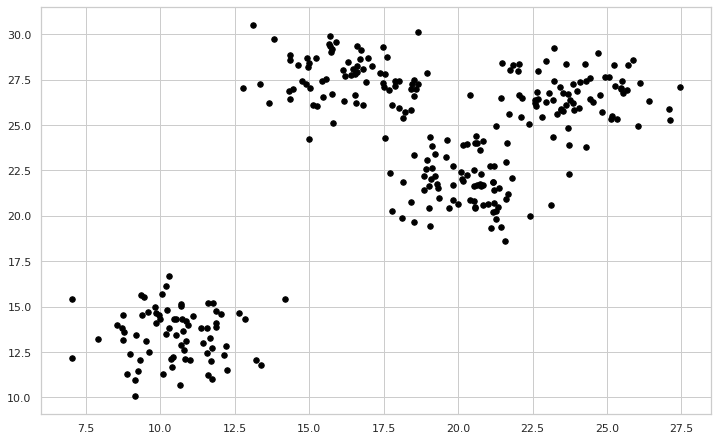
\includegraphics[width=0.6\textwidth]{img/fake_cluster.png}
		\caption{Diagrama de dispersão de dados fictícios.}
		\small \textsuperscript {Fonte: Elaboração própria}
		\label{fake_cluster}
	\end{figure}
	
	Existem dois objetivos possível de um método de agrupamento: agrupar as $n$ observações em um número desconhecido de grupos ou classificar as observações em um conjunto predefinido de grupos. No primeiro caso, a análise de agrupamento deve ser empregada, no segundo caso, a análise discriminante deve ser utilizada. Na análise de agrupamento, geralmente, o número de grupos não é conhecido a princípio e encontrar o melhor agrupamento não é uma tarefa simples (FERREIRA, 2011). 
	
	Bartholomew et al. (2008) apresenta duas etapas fundamentais em qualquer processo de agrupamento. A primeira é obter as distâncias de todos os pares de objetos para construção da matriz de proximidades. A segunda etapa consiste em desenvolver um algoritmo para formação de grupos com base nessas distâncias. 
	
	As distâncias, necessárias na primeira etapa, são determinadas com base em medidas de similaridade ou dissimilaridade. As medidas de dissimilaridade correspondem às distâncias, ao passo que as de similaridades complementam as distâncias, assim, quanto maior a medida de similaridade entre dois objetos menor será a de dissimilaridade e mais próximos eles serão (FERREIRA, 2011). A próxima seção apresenta algumas considerações a respeito de medidas de distâncias que podem ser utilizadas. 
	
	\subsubsection{Distâncias} 
	
	A realização de um procedimento de agrupamento necessita que se estabeleça \textit{a priori} uma medida de distância. Há diversas medidas de similaridade ou dissimilaridade entre pares de observações. Entre elas, as mais comuns são a distância euclidiana, distância euclidiana padronizada, Manhattan, Mahalanobis, etc. Essas medidas são de dissimilaridade, ou seja, quanto menor seus valores, mais próximos ou similares são os objetos comparados. É importante ressaltar que a escolha da métrica interfere diretamente no resultado final do agrupamento (MINGOTI, 2005; EVERITT et al., 2011). 
	
	A distância entre as observações $i$ e $j$ é paresentada na $i$-ésima linha e $j$-ésima coluna da matriz de distâncias. Por exemplo, se há $n = 4$ elementos na amostra, a matriz de distâncias terá dimensão $4$ $\times$ $4$ e será da forma
	
	\begin{align*}
	\left[
	\begin{array}{cccc}
	- & d_{12} & d_{13} & d_{14}\\
	d_{21} & - & d_{23} & d_{24}\\
	d_{31} & d_{32} & - & d_{34}\\
	d_{41} & d_{42} & d_{43} & -\\
	\end{array}
	\right],
	\end{align*}
	
	\noindent em que $d_{ij}$ é a distância entre os elementos $i$ e $j$. Geralmente, essa matriz é simétrica, ou seja, $d_{12}=d_{21}$, $d_{13}=d_{31}$, e assim por diante (BARTHOLOMEW et al., 2008).
	
	Uma das medidas de distância mais simples é a distância euclidiana, que pode ser calculada por 
	
	\begin{align*}
	d_{ij} = \sqrt{\sum_{k = 1}^{p}(X_{ik} - X_{jk})^2},
	\end{align*}
	
	\noindent em que $d_{ij}$ é a distância euclidiana entre os elementos $i$, com os valores $X_{i1}$, $X_{i2}$, $\dots$, $X_{ip}$, e $j$, com os valores $X_{j1}$, $X_{j2}$, $\dots$, $X_{jp}$.
	
	A distância de Mahalanobis e a euclidiana padronizada são generalizações da distância euclidiana. Sendo assim, a distância generalizada entre dois elementos $X_{i\cdot}$ e $X_{j\cdot}$ pode ser definida como  
	
	
	\begin{align}
	d_{ij} = (\boldsymbol{X}_{i\cdot} - \boldsymbol{X}_{j\cdot})^T \boldsymbol{A}(\boldsymbol{X}_{i\cdot} - \boldsymbol{X}_{j\cdot}). 
	\end{align}
	
	A escolha da matriz $\boldsymbol{A}$ define a distância a ser calculada. Quando $\boldsymbol{A}= \boldsymbol{I}$ obtém-se do cálculo a distâncias euclidiana, se $\boldsymbol{A}= \boldsymbol{D^{-1}}$ tem-se como resultado a distância euclidiana padronizada. Se $\boldsymbol{A}= \boldsymbol{S^{-1}}$, ou seja, a inversa da matriz de covariâncias dos dados, obtém-se a distância de Mahalanobis. Nesse último caso, o cálculo das distâncias leva em consideração as diferenças de variâncias e covariâncias entre as variáveis (MINGOTI, 2005). A medida de Mahalanobis, portanto, considera que objetos que possuem a mesma direção das correlações entre as variáveis sejam considerados mais similares entre si do que objetos situados em direções opostas. Além disso, essa medida de distância produz agrupamentos compactos e convexos e elimina o efeito de domínio na classificação das variáveis de maior variabilidade (FERREIRA, 2011).
	
	Após ser feita a definição da medida de distância a ser utilizada, o próximo passo da análise consiste em escolher um método de agrupamento. De acordo com Ferreira (2011), os métodos de agrupamento podem ser divididos em  em hierárquicos (aglomerativos ou divisivos) e não hierárquicos. No método hierárquico aglomerativo, o processo de agrupamento se inicia com $n$ grupos, cada um contendo uma observação, no final do método haverá um único grupo com todas as observações. A cada passo do processo iterativo, cada observação ou grupo é unido a outra observação ou grupo. A união se dá através de um critério de similaridade, os objetos mais próximos entre si são alocados para o mesmo grupo, até que, no final, todos estejam em um único grupo. Nos métodos hierárquicos divisivos, ocorre o processo contrário. No início há um único grupo com as $n$ observações e, ao final, haverá $n$ grupos, cada um com uma observação. Nos métodos não hierárquicos é necessário definir o número de grupos $(k)$ \textit{a priori} para que, em seguida, se possa atribuir as $n$ observações aos $k$ grupos da melhor maneira possível. No início do processo utiliza-se uma alocação arbitrária e, iterativamente, busca-se a alocação ótima.
	
	\subsubsection{Técnicas hierárquicas aglomerativas}
	
	Ao se utilizar o método hierárquico aglomerativo, depois que uma fusão é realizada, ela não será mais desfeita. Assim, quando o método coloca dois elementos em um mesmo grupo, eles não mais aparecerão em grupos diferentes. Para o pesquisador encontrar a melhor solução com o número de agrupamentos ótimo, ele deverá adotar algum critério de divisão (EVERITT; HOTHORN, 2011).
	
	Agrupamentos obtidos a partir de métodos hierárquicos, aglomerativos ou divisivos, podem ser representados por um diagrama bidimensional muito utilizado, o dendrograma. Esse gráfico ilustra as fusões ou divisões realizadas a cada passo do processo. Maiores detalhes podem ser obtidos em (EVERITT et al., 2011).
	
	Dentre os métodos hierárquicos aglomerativos o método de Ward, ou método da mínima variância, se fundamenta na mudança de variação entre os grupos e também dentro dos grupos que são formados em cada passo do agrupamento. A cada passo de agrupamento é calculada a soma de quadrados dentro dos grupos. Tal soma consiste no quadrado da distância euclidiana de cada elemento amostral pertencente ao grupo em relação à seu respectivo vetor de médias. O método de Ward se assemelha ao método do centroide no que se refere a utilização dos vetores de médias amostrais, porém a distância utilizada no método de Ward leva em consideração os tamanhos dos grupos que estão sendo comparados. A soma de quadrados dentro do $i$-ésimo grupo é definida como:  
	\begin{align*}
	SQDG_i = \sum_{j=1}^{n_i}(X_{ij} - \bar{X}_{i})^2,
	\end{align*}
	sendo $n_i$ o número de elementos no grupo $i$, $X_{ij}$ o vetor de observações do $j$-ésimo elemento amostral pertencente ao $i$-ésimo agrupamento e $\bar{X}_{i}$ o centroide do $i$-ésimo agrupamento, representando a soma de quadrados correspondente a tal grupo.
	
	A distância entre dois grupos quaisquer, $G_i$ e $G_l$, é definida como:
	\begin{align*}
	d_{ G_i,G_l} = \left(\dfrac{n_l n_i}{n_l + n_i}\right)(X_{ij} - \bar{X}_{i})^2.			
	\end{align*}
	
	Em cada passo do agrupamento, os dois grupos que minimizam tal distância são combinados. Tal método tende a produzir grupos com aproximadamente o mesmo número de elementos e é apropriado somente a variáveis quantitativas por ter como base de comparação o vetor de médias amostral (MINGOTI, 2005).
	
	\subsubsection{Técnicas não hierárquicas: \textit{K}-médias}
	
	Nos métodos não hierárquicos, se dois objetos forem unidos em algum passo do  processo, pode ser que eles não permaneçam no mesmo grupo na partição final.  Como consequência, não é possível construir dendrogramas para a representação dos agrupamentos formados a cada passo (MINGOTI, 2005). Há diversos métodos não hierárquicos, como métodos baseados em estimação de densidades, misturas de distribuição e partição. Entretanto, os procedimentos de partição são os mais utilizados e, entre eles, o das k-médias é o mais popular (FERREIRA, 2011).
	
	A técnica de agrupamento das $k$-médias (\textit{k-means}) procura uma partição das $n$ observações em $k$ agrupamentos ($G_1$, $G_2$, $\cdots$, $G_k$), em que $G_i$ denota o conjunto de observações que está no $i$-ésimo grupo e $k$ é dado por algum critério numérico de minimização. A implementação mais usada do método tenta encontrar a partição dos $n$ elementos em $k$ grupos que minimize a soma de quadrados dentro dos grupos ($SQDG$) em relação a todas as variáveis. Esse critério pode ser escrito como 
	\begin{align*}
	SQDG = \sum_{j=1}^{p}\sum_{l=1}^{k}\sum_{i \in G_l}(X_{ij} - \bar{X}_{j}^{(l)})^2,
	\end{align*}
	em que $\bar{X}_{j}^{(l)} = \displaystyle\frac{1}{n_i}\sum_{i \in G_l}X_{ij}$ é a média dos indivíduos no grupo $G_l$ em relação à variável $j$ (EVERITT; HOTHORN, 2011).
	
	Ainda de acordo com os autores, apesar de o problema parecer relativamente simples, ele não é tão direto. A tarefa de selecionar a partição com a menor soma de quadrados dentro dos grupos se torna complexa porque o número de partições possíveis se torna muito grande mesmo com um tamanho amostral não tão grande. Por exemplo, para $n = 100$ e $k=5$, o número de partições é da ordem de $10^{68}$. Esse problema levou ao desenvolvimento de algoritmos que não garantem encontrar a solução ótima, mas que levam a soluções satisfatórias.
	
	% \subsubsection{Número de grupos}
	
	\subsection{Análise Espacial}
	
	A análise espacial consiste em um conjunto de métodos capazes de mensurar propriedades e relacionamentos de acordo com a localização espacial de determinado fenômeno. Ou seja, um conjunto de técnicas que tem como objetivo a incorporação do espaço à análise. Dessa forma, antes de partir para a modelagem, é comumente  realizada a análise exploratória dos dados, buscando identificar os padrões de dependência espacial no fenômeno em questão (CÂMARA et al., 2002).
	
	Dentre os principais fenômenos espaciais incorporados à análise, estão a dependência espacial e a heterogeneidade espacial. O fenômeno da dependência espacial pode ser representado pela Primeira Lei da Geografia, ou Lei de Tobler. Tal lei foi enunciada no ano de $1970$ pelo geógrafo suíço Waldo Tobler e diz que tudo depende de tudo, mas coisas próximas estão mais relacionadas entre si do que coisas mais distantes. Sendo assim, a dependência espacial consiste no fato de que o valor de uma variável em uma certa região depender do valor desta mesma variável nas regiões próximas (ALMEIDA, 2012).
	
	Ainda segundo Almeida (2012), processos temporais possuem relações diferentes dos processos espaciais. No sentido que, no primeiro deles o valor de uma variável qualquer no tempo $t$ é influenciado pelo valor da variável no tempo $t-1$, mas o inverso não ocorre. Diferentemente desse tipo de processo, nos  processos espaciais têm-se a multidirecionalidade nas relações entre as regiões, ou seja, o valor da variável na região $i$ depende do valor na região $j$, e a região $j$ depende da região $i$ em relação ao valor da mesma variável.
	
	%Heterogeneidade Espacial
	
	O relacionamentos espaciais incorporados à análise, a heterogeneidade espacial, refere-se à variação nos relacionamentos entre as variáveis ao longo do espaço. Em geral, podem-se esperar diferentes relacionamentos em cada uma das unidades espaciais, podendo a relação linear entre tais unidades ser escrita como:
	
	\begin{align*}
	y_i = X_i \beta_ i + \epsilon_i,
	\end{align*}
	
	\noindent em que $i$ é o índice da observação no espaço, assumindo valores de 1 a \textit{n}, $X_i$ representa o vetor contendo os \textit{k} valores da variável explicativa, tendo um conjunto de parâmetros associados $\beta_i$.
	
	É importante ressaltar que os dados espaciais possuem alguns problemas que podem ser danosos à análise. Além da heterogeneidade espacial e da dependência espacial, é possível citar problemas como a falácia ecológica, o problema da unidade de área modificável, o efeito de beirada e a influência de \textit{outliers} espaciais. 
	
	De acordo com Almeida (2012), a falácia ecológica está relacionada com erros que se originam ao deduzir o comportamento do indivíduo através análise de dados agregados. Almeida (2012) argumenta que há razões para inferir, ainda que parcialmente, comportamentos individuais por meio de dados agregados. Uma situação possível é quando alguns comportamentos individuais são influenciados pelo comportamento do grupo. No entanto, via de regra, as conclusões a respeito de comportamento individual devem se basear primordialmente em dados individuais. 
	
	Outro problema que surge no contexto da análise espacial é o  problema de unidade de área modificável, usualmente denotado pela sigla MAUP, do inglês \textit{modifiable areal unit problem}. Esse problema se refere, basicamente as consequências causadas pelas diferentes formas de se delimitar as unidades espaciais. A necessidade de agregação de informações espaciais se dá pela ausência de dados individuais, ou então quando as unidades agregadas são o objeto da análise.
	
	Segundo Haining (2003), o MAUP apresenta dois efeitos distintos, o problema de escala e o de partição. O primeiro deles se relaciona à escala da análise, ou seja, ao número de subáreas em que a região de estudo foi particionada. O número de partições determina também o tamanho de cada unidade espacial nas quais os eventos são observados, portanto é capaz de influenciar o resultado de estatísticas. O segundo efeito diz respeito a forma das partição das unidades, ou seja, como as  áreas estão divididas mantendo-se constante o  o número de áreas.
	
	O efeito de beirada se deve a possibilidade da dependência espacial ir além das fronteiras da região de estudo, podendo o valor da variável mensurada depender de outras unidades espaciais que não fazem parte da mesma (ANSELIN, 1988). Tal efeito interfere na  inferência estatística de modelos de processos espaciais. Além disso, Almeida (2012) aponta que, por terem um menor número de regiões vizinhas, as regiões da fronteira também fornecem menos informação para a construção de valores médios, como por exemplo as defasagens espaciais.
	
	Para lidar com o efeito beirada, Griffith (1983) propôs a criação de vizinhos artificiais para as regiões de fronteira por meio da replicação do mapa. Desta forma, as regiões da beirada oposta da área de estudo seriam também vizinhas da outra beirada. Porém, como destacado por Darmofal (2006) a dúvida seria saber se tais vizinhos artificiais realmente apresentam interação espacial com a região. Outra solução apontada por Almeida (2012) seria estender a área de estudos, considerando adicionalmente uma zona ao longo de toda a fronteira.
	
	%Outliers e pontos de alavancagem
	Por fim, os \textit{outliers} espaciais são definidos como valores extremos com relação a suas posições no mapa. A presença de \textit{outliers} espaciais se dá considerando a dissimilaridade dos valores relação ao conjunto de valores das regiões vizinhas (HAINING, 2003). Os \textit{outliers} espaciais e os pontos de alavancagem podem surgir de do processo de obtenção e armazenamento dos dados, porém não são somente essas suas origens. Tais valores podem realmente sinalizar a presença de valores extremos e representar características reais do fenômeno em estudo. Portanto a presença de \textit{outliers} espaciais implica a necessidade de uma investigação mais cautelosa (ALMEIDA, 2012)
	
	\subsubsection{Matriz de Ponderação Espacial}
	
	
	Uma matriz de ponderação espacial tem como objetivo representar um determinado arranjo espacial das interações resultantes de um fenômeno em estudo (ALMEIDA, 2012). Nessa matriz cada conexão entre duas regiões é representada por uma entrada na matriz que é denominada peso espacial. A matriz de ponderação espacial é, geralmente, denotada por \boldsymbol{$W$}: 
	
	\begin{align*}
	\boldsymbol{W} =
	\left[
	\begin{array}{cccc}
	w_{11} & w_{12} & \dots & w_{1n} \\
	w_{21} & w_{22} & \dots &w_{2n} \\
	\vdots & \vdots & \ddots & \vdots \\
	w_{n1} & w_{n2} & \dots & w_{nn}\\
	\end{array}
	\right],
	\end{align*}
	
	\noindent com dimensão $n \times n$, em que $n$ é o número de regiões em análise. Cada elemento $w_{ij}$ representa uma medida de proximidade entre as áreas $i$ e $j$ (CÂMARA et al. 2002). 
	
	Existem dois problemas relacionados a determinação da matriz de ponderação espacial a ser utilizada. O primeiro está relacionado ao fato de que, muitas vezes a escolha da matriz $\boldsymbol{W}$ é arbitrária, pois não existe teste formal para sua escolha. O segundo problema, está relacionado a sensibilidade dos resultados à escolha da matriz. Portanto, a definição da matriz de ponderação espacial tem grande importância e deve levar em consideração uma fundamentação teórica (ALMEIDA, 2012). 
	
	Em sua maioria, os modelos tradicionais, utilizam atributos físicos e geográficos para estabelecer distâncias entre as regiões. Comumente são utilizados critérios como a vizinhança, a distância geográfica ou tempo de deslocamento entre as unidades. Entretanto, em modelos espaciais aplicados a políticas públicas, é possível que as distâncias entre as regiões busquem representar mais aspectos socioeconômicos do que geográficos \cite{tyszler06}. 
	
	Ao definir uma matriz de ponderação espacial por contiguidade são levadas em consideração as fronteiras físicas em comum entre duas regiões. Em sua forma binária, dado que tais regiões apresentam relação de vizinhança, é atribuído ao elemento correspondente na matriz o valor $1$, caso contrário é atribuído o valor $0$. Formalmente, tem-se:
	
	\[
	w_{ij} = 
	\begin{cases}
	\text{1,} & \quad\text{se $i$ e $j$ são contíguos} \\
	\text{0,} & \quad\text{se $i$ e $j$ não são contíguos.}\\
	\end{cases}
	\]
	\\
	
	Por convenção assume-se que  $w_{ij} =  0$, para todo $i = j$, ou seja, uma determinada região não é considerada vizinha de si própria. Porém, é possível encontrar na literatura com menor frequência regiões sendo vizinhas de si mesmas. Além disso, o conceito de fronteira geográfica pode apresentar diferentes definições na observação de um mapa, para isso, o movimento de peças em um tabuleiro de xadrez é utilizado para denominar algumas das diferentes convenções de contiguidade (ALMEIDA, 2012).
	
	Na Figura \ref{contiguidade} são representadas três diferentes convenções de contiguidade: rainha (\textit{queen}), torre (\textit{rook}) e bispo (\textit{bishop}), respectivamente. Na primeira delas, além das regiões que fazem fronteira com a região $A$, os vértices são considerados vizinhos. Na convenção torre, apenas as regiões que fazem fronteira com a região são consideradas vizinhas de $B$. No último caso, apenas os vértices são considerados vizinhos da região $C$.
	
	\begin{figure}[h!]
		\centering
		\small
		\subfloat[Rainha\label{fig:a}]{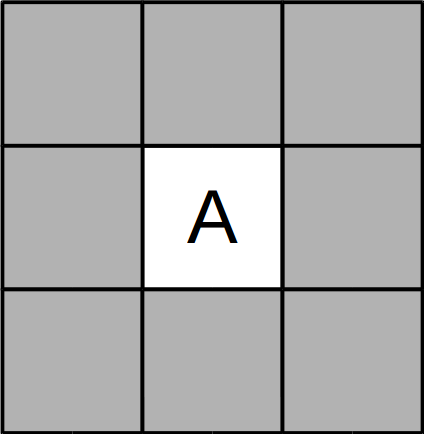
\includegraphics[width=0.15\textwidth]{img/cont_queen.png}}\hspace{0.2cm}
		\subfloat[Torre\label{fig:b}]{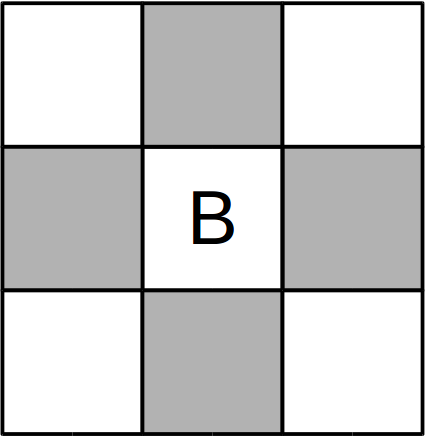
\includegraphics[width=0.15\textwidth]{img/cont_rook.png}}\hspace{0.2cm}
		\subfloat[Bispo\label{fig:c}]{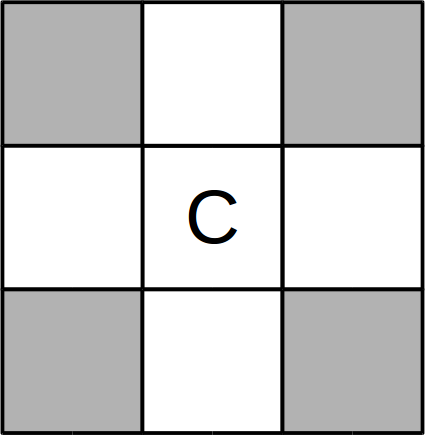
\includegraphics[width=0.15\textwidth]{img/cont_bishop.png}}
		\caption{Convenções de contiguidade}
		\small \textsuperscript {Fonte: Elaboração própria}
		\label{contiguidade}
	\end{figure}
	
	
	É importante destacar que a matriz de contiguidade binária é simétrica, no sentido que se duas regiões quaisquer $i$ e $j$ compartilham fronteiras físicas, tanto $w_{ij}$ quanto $w_{ji}$ serão iguais a 1. Deste modo, a influência exercida pela região $i$ em $j$ será observada na relação entre $j$ e $i$, o que ilustra o conceito de multidirecionalidade da influência no espaço. Vale ressaltar que, após a normalização nas linhas da matriz de ponderação espacial (divisão de cada elemento pela soma da linha), a matriz resultante não necessariamente será simétrica.
	
	
	As matrizes que utilizam as distâncias geográficas como critério para a definição dos pesos consideram que duas regiões próximas geograficamente apresentam maior interação espacial. Dentre as matrizes com essa definição, a matriz dos $k$ vizinhos mais próximos é uma das mais utilizadas. Na Equação \ref{W_prox}, $d_i(k)$ representa a menor distância em relação a região $i$ para que $i$ tenha exatamente $k$ vizinhos \cite{almeida12}.
	
	\begin{align}
	w_{ij} = 
	\begin{cases}
	\text{$1,$} & \quad\text{se $d_{ij} < d_i(k)$} \\
	\text{$0,$} & \quad\text{se $d_{ij} > d_i(k)$}\\
	\end{cases}
	\label{W_prox}
	\end{align}
	
	De acordo com Almeida (2012), a matriz de pesos espaciais gerais de Cliff e Ord  estabelece que, duas regiões que compartilham maior extensão de fronteira apresentam uma maior interação entre si, além de considerar o fator de distância entre as regiões. Ambas as informações são utilizadas no cálculo dos pesos da matriz, sendo esses definidos pelo comprimento relativo da fronteira comum entre as regiões, ajustados pela distância inversa entre elas. Os pesos espaciais da matriz de pesos gerais são expressos da seguinte maneira:
	
	\begin{align*}
	w_{ij} = \frac{f_{ij}^\phi}{d_{ij}^\delta},
	\end{align*}
	
	\noindent em que $f_{ij}$ é a proporção da fronteira comum entre as observações $i$ e $j$ no perímetro de $i$, e $\phi$ e $\delta$ são parâmetros a serem definidos. Tal matriz de pesos espaciais não necessariamente será simétrica. Ao levar em consideração a proporção do perímetro total da região $i$ que é comum a região $j$ em regiões de diferentes perímetros, tal proporção também seria distinta.
	
	
	\subsubsection{Análise Exploratória de Dados Espaciais}
	
	A análise exploratória de dados espaciais (AEDE) tem objetivo de descrever como estão distribuídas espacialmente as observações buscando compreender seus padrões de associação espacial e verificar a existência de \textit{clusters} espaciais. Além disso, a AEDE busca analisar se existem diferentes regimes espaciais  ou quaisquer formas de instabilidade, juntamente com a identificação de observações atípicas, ou como são também denominados, \textit{outliers} espaciais (ALMEIDA, 2012).
	
	A necessidade de se utilizar metodologias exploratórias de dados espaciais se dá pois, como afirmam Messner et al. (1999, p. 427), “a percepção humana não é suficientemente rigorosa para determinar agrupamentos significativos e, de fato, tende a ser enviesada para achar padrões, mesmo em dados espaciais aleatórios.” Por meio destas metodologias, é possível utilizar indicadores de associação espacial globais ou locais com o objetivo de identificar os diferentes regimes espaciais do conjunto de dados.
	
	Exemplos de padrões de autocorrelação espacial são apresentados na Figura \ref{autocorrelacao}. É possível identificar em (a) um padrão de autocorrelação positivo, ou seja, valores semelhantes estão localizados próximos uns dos outros. Em (b) é apresentado uma autocorrelação nula, o que indica que há uma aleatoriedade da distribuição espacial do atributo. Por sua vez, em (c), há um padrão de autocorrelação negativo, indicando que valores dissimilares se encontram próximos uns dos outros. 
	
	\begin{figure}[h!]
		\centering
		\small
		\subfloat[Positiva\label{fig:a1}]{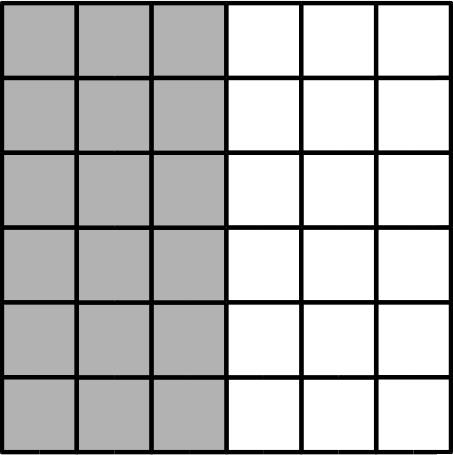
\includegraphics[width=0.15\textwidth]{img/autocor_pos.png}}\hspace{0.2cm}
		\subfloat[Nula\label{fig:b2}]{
\includegraphics[width=0.15\textwidth]{img/autocor_null.png}}\hspace{0.2cm}
		\subfloat[Negativa\label{fig:c2}]{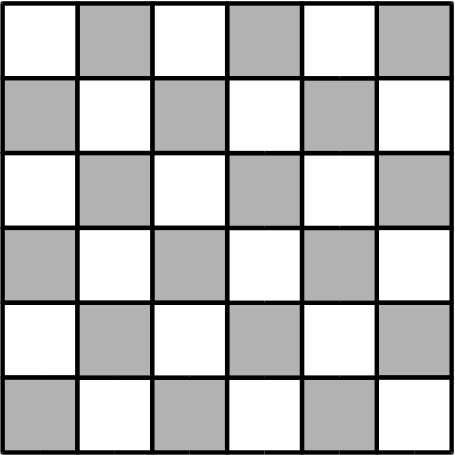
\includegraphics[width=0.15\textwidth]{img/autocor_neg.png}}
		\caption{Padrões de autocorrelação espacial}
		\small \textsuperscript {Fonte: Elaboração própria}
		\label{autocorrelacao}
	\end{figure}
	
	A Figura \ref{autocorrelacao}, apresenta dados no formato de \textit{grids} regulares, no entanto, geralmente as regiões em estudo são polígonos irregulares. Este fato, dificulta a identificação visual, principalmente dos padrões de autocorrelação nula e negativa. Tornando, então,	 necessário a utilização de testes estatísticos para a identificação dos padrões de autocorrelação espacial. 
	
	\subsubsection{Autocorrelação Espacial Global}
	
	O coeficiente I de Moran, proposto em 1948, é um dos principais indicadores de autocorrelação espacial global \cite{almeida12}. Tal coeficiente é expresso por meio medida de auto-covariância na forma de produto cruzado. A forma algébrica da estatística é dada por:
	
	\begin{align}
	\label{IMoran}
	I = \dfrac{n}{S_0} \dfrac{\sum_{i} \sum_{j} w_{ij} z_i z_j}{\sum_{i=1}^{n} z_i^2}.
	\end{align}
	
	\noindent em que $n$ representa o número de regiões, $z_i$ denota o valor da variável de interesse padronizada na região $i$ e $S_0$ é  o somatório de todos os pesos espaciais da matriz \boldsymbol{$W$} \cite{almeida12}:
	
	Matricialmente, tal coeficiente pode ser calculado pela da seguinte forma:
	
	\begin{align*}
	I = \dfrac{n}{S_0} \dfrac{z'\boldsymbol{W}z}{z'z},
	\end{align*}
	
	\noindent em que $\boldsymbol{W}z$ representa os valores médios da variável padronizada nos vizinhos de acordo com a matriz \boldsymbol{$W$}.
	
	O \textit{I} de Moran é utilizado, de forma geral, para testar a presença de autocorrelação espacial, sendo a aleatoriedade espacial a hipótese nula do teste. Cliff e Ord (1981) demonstraram que o \textit{I} de Moran não é centrado em $0$, mas sim em seu valor esperado $-[1/(n-1)]$, que é o valor que seria obtido em uma situação de aleatoriedade na distribuição espacial. Dessa forma, valores da estatística entre o valor esperado e $1$ indicam autocorrelação espacial positiva, valores entre $-1$ e o valor esperado indicam autocorrelação espacial negativa. 
	
	A autocorrelação espacial positiva indica que no geral, as regiões que apresentam valores altos na variável de interesse tendem a ter ao seu redor regiões que também apresentam valores altos desta variável e regiões com baixos valores tendem a estar circundadas por regiões que também apresentam baixos valores. Por outro lado, a autocorrelação espacial negativa indica dissimilaridade entre os valores da variável de interesse e a localização dos mesmos. Nesse sentido, geralmente regiões com valores altos da variável estão rodeadas por regiões com baixos valores e regiões com baixos valores têm ao seu redor regiões com valores altos (ALMEIDA, 2012).
	
	Após o cálculo do índice I de Moran, é necessário verificar se a correlação espacial representada pelos valores é significativa. Tal verificação pode ser obtida pela associação do índice a uma distribuição estatística, geralmente  a distribuição normal. A abordagem mais utilizada para tal verificação é o teste de pseudo-significância, sem pressupostos em relação à distribuição. Em tal abordagem são geradas diferentes permutações dos valores associados às regiões, produzindo assim para cada permutação um novo arranjo espacial com os valores redistribuídos entre as áreas. Dado que a situação observada corresponde somente a apenas um dos arranjos, tem-se uma distribuição empírica do índice \cite{camara04}. Tal abordagem também é conhecida como teste de permutação aleatória.
	
	O diagrama de dispersão de Moran, exemplificado na Figura \ref{dispersaomoran}, consiste em outra forma de visualizar os regimes espaciais dos dados em questão. Em seu eixo horizontal, são representados os valores padronizados da variável de interesse, já no eixo vertical estão as médias da variável nos vizinhos das respectivas áreas.
	
	
	\begin{figure}[H]
		\centering
		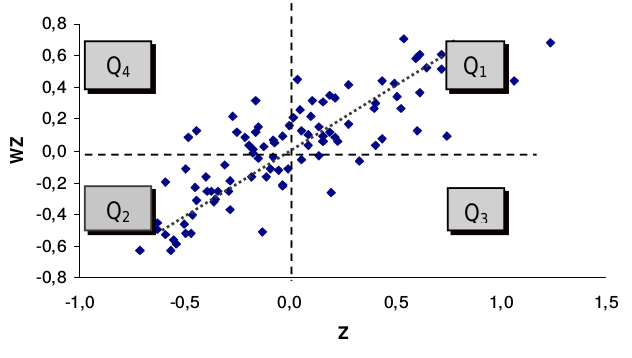
\includegraphics[scale = 0.5]{img/dispersaoMoran.png}
		\vspace{-0.4cm}
		\caption{Diagrama de dispersão de Moran}\label{dispersaomoran}
		\small \textsuperscript {Fonte: Câmara et al. (2002)}
	\end{figure}
	
	
	%\begin{figure}[h!]
	%	\centering
	%	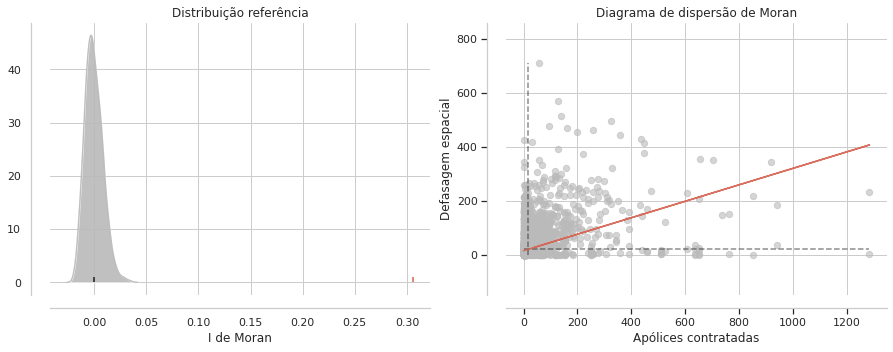
\includegraphics[width=0.8\textwidth]{img/i_de_moran.png}
	%	\caption{\textit{I} de Moran para Apólices contratadas}
	%	\footnotesize{Fonte: Elaboração própria}
	%	\label{fig:1}
	%\end{figure}
	
	%%%%%%%%%%%%%%% G de Getis & Ord  %%%%%%%%%%%%%%% 
	
	
	\subsubsection{Autocorrelação Espacial Local}
	
	
	%%%%%%%%%%%%%%% G de Getis & Ord local  %%%%%%%%%%%%%%% 
	
	De forma pioneira Getis e Ord propuseram, em 1992, criar um indicador de concentração espacial para analisar localmente a associação espacial (ALMEIDA, 2012). Segundo Getis e Ord (1992), essa estatística tem a capacidade de alertar o pesquisador para presença de eventuais bolsões localizados de concentração espacial, chamados de \textit{hot spot} e \textit{cool spots}. A estatística proposta indica, para cada observação $i$, em que medida essa observação está rodeada por valores altos (\textit{hot spot}) ou baixos (\textit{cool spot}). A estatística, para uma determinada variável, é calculada da seguinte forma 
	
	\begin{equation}
	G_i(d) = \dfrac{\sum_{j} w_{ij}(d) y_j}{\sum_{j}  y_j},\quad \text{para  $j \neq i$}
	\label{g_getis_ord_l}
	\end{equation}
	
	\noindent em que $y$ é a variável de interesse. O somatório em $j$ faz com que apenas os valores dos vizinhos próximos da região $i$ sejam utilizados no cálculo da estatística. A matriz de ponderação espacial $\boldsymbol{W}$ pode ou não ser uma matriz de proximidade geográfica, baseada em um raio construído em torno da região $i$, como na Equação \ref{W_prox}. 
	
	Há duas possibilidades para a estatística $G$ de Getis e Ord, se não incluir a observação sob consideração $i$, tem-se a estatística $G_i$ como apresentada da definição \ref{g_getis_ord}. Se incluir a observação $i$ no somatório, obtém-se $G_i^*$ que é expressa como: 
	
	\begin{equation}
	G^*(d) = \dfrac{\sum_{j} w_{ij}(d) y_j}{\sum_{j}  y_j},\quad \text{para qualquer } j.
	\label{g_getis_ord}
	\end{equation}
	
	A média da estatística $G_i$ é dada por 
	
	\begin{equation*}
	\mathbb{E}(G) = \dfrac{W_i}{(n-1)}  
	\end{equation*}
	
	\noindent em que $W_i = \sum_j x_{ij}(d)$Ward
	
	A variância da estatística $G_i$ é dada por  
	
	\begin{equation}
	Var(G_i)= \dfrac{W_i(n-1-W_i)}{(n-1)^2(n-1)} \bigg[\dfrac{s(i)}{\bar{y}(i)}\bigg]^2
	\end{equation}
	
	\noindent em que $\bar{y}(i)= \dfrac{\sum_j y_j}{(n-1)}$ e $s^2(i) = \dfrac{\sum_j y_j^2}{(n-1)} - [\bar{y}(i)]^2$. 
	
	A inferência a respeito da significância da estatística $G_i$ é baseada na normal padrão, ou seja $Z(G_i)$. A interpretação é feita com base no sinal de $Z(G_i)$, valores positivos e significativos indicam um \textit{cluster} espacial do tipo \textit{hot spot}, ou seja com valores altos para a variável de interesse. Por outro lado, um valor negativo e significativo de $Z(G_i)$ indica um \textit{cluster} do tipo \textit{cool spot}, ou seja de baixos valores para a variável de interesse (ALMEIDA, 2012). 
	
	É necessário ressaltar que esse indicador não é capaz de indicar um padrão espacial de dispersão da variável, ou seja, uma situação de correlação negativa. A estatística $G_i$ de Getis e Ord só é capaz de fornecer informação sobre o padrão espacial de concentração, ou seja, \textit{hot spot} ou \textit{cool spot}. Padrões de concentração espacial do tipo Alto-Baixo (AB) ou Baixo-Alto (BA) não são capturados por esse indicador. Também é importante ressaltar que o indicador de Getis e Ord não pode ser calculado para valores negativos da variável.  Além disso, nessa versão do indicador, a matriz $\boldsymbol{W}$ utilizada  tem que ser simétrica e com pesos binários (ALMEIDA, 2012). 
	
	Para permitir o calculo da estatística $G_i$ com valores negativos e com a possibilidade de uma matriz de pesos não simétrica, Getis e Ord (1995) propuseram uma nova estatística $(NG_i)$, obtida a partir da padronização de $G_i$. A estatística $(NG_i)$ é expressa como 
	
	\begin{equation}
	NG_i = \dfrac{G_i-\mathbb{E}(G_i)}{DP(G_i)}
	\end{equation}
	\noindent em que $\mathbb{E}(G_i)$ é a média teórica de $G_i$ e $DP(G_i)$ é o desvio padrão de $G_i$ (ALMEIDA, 2012).
	
	%%%%%%%%%%%%%%%  I de Moram Local %%%%%%%%%%%%%%% 
	
	Proposto por Anselin em 1995, outro indicador com a capacidade de detectar padrões locais de autocorrelação espacial, estatisticamente significativos, é o $I_i$ de Moran local (ALMEIDA, 2012). Segundo Anselin (1995), um indicador com capacidade de detectar padrões locais de autocorrelação espacial é chamado \textit{``local indicator of spatial association} (LISA)" e deve satisfazer dois critérios: 
	
	\begin{enumerate}
		\item para cada observação, o indicador, deve ser capaz de indicar \textit{clusters} espaciais estatisticamente significativos;
		\item o somatório dos indicadores locais, calculados para todas as regiões, deve corresponder ao indicador de autocorrelação espacial global para as mesmas regiões.
	\end{enumerate}
	
	O $I_i$ de Moran local decompõe o $I$ de Moran global em quatro categorias: Alto-Alto (AA), Baixo-Baixo (BB), Alto-Baixo (AB) e  Baixo-Alto (BA). Essas categorias correspondem aos quadrantes do diagrama de dispersão de Moran (Figura \ref{dispersaomoran}). A estatística $I_i$ de Moran local para a variável padronizada $z_i$, observada na regão $i$, pode ser expressa como 
	
	\begin{align*}
	I_i = z_i \sum_{j}^{} w_{ij} z_j,
	\end{align*}
	
	O cálculo de $I_i$ é feito incluindo apenas as regiões vizinhas de $i$, definidas através da matriz de pesos espaciais. Para cada observação $n$ obtém-se um valor de $I_i$ que gera uma grande quantidade de informação. Uma forma mais eficiente de visualizar o conjunto de estatísticas geradas pelo $I_i$ de Moran local é apresenta-los em um mapa de \textit{clusters}. Esse mapa combina informação do diagrama de dispersão de Moram (Figura \ref{dispersaomoran}) com a significância da medida de associação local $I_i$ (ALMEIDA, 2012). 
	
	Para exemplificar na Figura \ref{lisa_ex} é apresentado um mapa de \textit{clusters} \textit{LISA} para apólices de seguro rural contratadas nos municípios do Brasil. Como é possível observar, o mapa da Figura \ref{lisa_ex} ilustra a classificação em quatro categorias de associação espacial estatisticamente significativas. 
	
	\begin{figure}[h!]
		\centering
		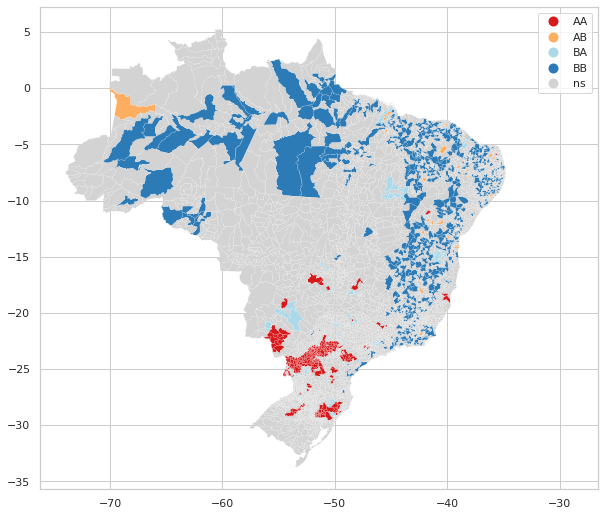
\includegraphics[width=0.6\textwidth]{img/liza_ex.png}
		\caption{Mapa de \textit{clusters LISA} para apólices contratadas de seguro rural}
		\small \textsuperscript {Fonte: Elaboração própria}
		\label{lisa_ex}
	\end{figure}
	
	Ambas as estatísticas de autocorrelação espacial local, $G_i$ e $I_i$, apresentam vantagens e desvantagens. Uma vantagem do $G_i$, em relação ao $I_i$, é a capacidade de estabelecer uma definição mais clara de \textit{clusters} com valores altos  (\textit{hot spot}) ou \textit{clusters} com valores baixos (\textit{cool spots}). Entretanto, valores negativos de $I_i$ indicam uma associação espacial de valores dissimilares, ou seja, valores baixos da variável, circundados por valores altos ou valores altos circundados por valores baixos. Esse tipo de associação não é captado pelo $G_i$, ou seja essa estatística não possui a capacidade de revelar \textit{outliers} globais (DARMOFAL, 2006).
	
	
	\newpage
	\section{Material e Métodos}\label{metodologia}
	
	O objetivo dessa seção é apresentar os dados utilizados no trabalho e descrever a metodologia e os recursos computacionais utilizados na presente análise.
	
	\subsection{Dados}
	
	% Quais os dados 
	Esse trabalho trabalho utilizará dados referentes a apólices de seguro rural dos municípios brasileiros no ano de 2018. As variáveis a serem utilizadas, bem como suas siglas e descrições, são apresentadas na Tabela \ref{variaveis}.
	
	% Quais as variáveis
	
	\begin{table}[!htp]
		\caption{Descrição das variáveis utilizadas.} 
		\footnotesize
		\vspace{0.1cm}
		\label{variaveis}
		\begin{tabularx}{\textwidth}{lXX}
			\hline \\[-1.8ex]	 
			Sigla            & Variável                                              \\ \hline
			apo\_cont        & Total de apólices contratadas                         \\
			seg\_t\_mil      & Soma da importância segurada (R\$ milhão)             \\
			premio\_t\_mil   & Soma dos prêmios (R\$ milhão)                         \\
			subv\_t\_mil     & Total de subvenção (R\$ milhão)                       \\
			indeniz\_mil     & Soma das indenizações pagas (R\$ milhão)              \\
			sinist\_media    & Total de sinistros pagos / total do prêmio arrecadado \\ 
			taxa\_media      & Taxa média aplicada às apólices                       \\
			apo\_indeniz     & Número de apólices indenizadas                        \\ 
			centroide        & Centroides das regiões dos municípios                 \\ \hline
		\end{tabularx}
		\footnotesize{Fonte: Elaboração própria}
	\end{table}
	
	
	% Fonte dos Dados 
	Os dados utilizados nesse trabalho sobre seguro rural estão disponíveis no endereço eletrônico do Ministério da Agricultura, Pecuária e Abastecimento (MAPA). Os centroides serão calculados a partir de dados que contém atributos geográficos, como a posição e o formato, do território brasileiro. Esses dados estão disponíveis no endereço eletrônico do Instituto Brasileiro de Geografia e Estatística (IBGE, 2020).
	
	%Padronização
	Como as variáveis estão em diferentes escalas e, com isto possuem diferentes variâncias, será realizada a padronização das variáveis para que tais fatores não interfiram na análise. Tal padronização será	 efetuada subtraindo-se de cada observação a média de sua respectiva variável e dividindo-se posteriormente pelo desvio padrão da variável.
	
	\subsection{Metodologia}
	
	Inicialmente será realizada uma análise exploratória dos dados que auxiliará na aplicação das técnicas de agrupamento. Após a etapa de formulação do problema, escolha das variáveis e análise exploratória dos dados, será aplicada a técnica de componentes principais componentes principais (ACP) com o objetivo de reduzir a dimensionalidade dos dados. O método será aplicado com a intenção de reduzir o conjunto das variáveis originais correlacionadas entre si a um novo conjunto de variáveis, os componentes principais (CPs), não correlacionadas. Os escores, valores numéricos dos componentes, do primeiro componente principal serão utilizados para a análise multivariada e para a análise exploratória de dados espaciais. 
	
	O próximo passo consiste na aplicação da técnica multivariada de análise de agrupamento para identificar os grupos de municípios brasileiros com características semelhantes em relação a variáveis de seguro rural, representadas 	pelos escores do primeiro CP. Nesse sentido, o primeiro passo consiste selecionar qual seria o método de agrupamento mais adequado para classificar os municípios. Nesse caso opta-se por escolher o método não hierárquico das $k$-médias que demonstra um desempenho superior aos métodos hierárquicos (MOOI; SARSTEDT, 2011). Em linhas gerais, com o uso dessa técnica, cada município será alocado no grupo cujo vetor de médias amostral será o mais semelhante ao vetor de valores observados para o respectivo município (MINGOTI, 2005).
	
	O método das $k$-médias exige que seja definido \textit{a priori} tanto o número de grupos desejado quanto os $k$ centroides iniciais. Para a definição do número de grupo será feito o uso de uma técnica hierárquica aglomerativa. Nessa abordagem, uma técnica hierárquica é aplicada para identificar o número de grupos \textit{a priori} e, em seguida, são definidas as sementes iniciais, o que possibilita a aplicação do método das $k$-médias para classificar as observações.
	
	Neste trabalho, será empregado o método de Ward para especificar o número de grupos pretendido. Além de retornar melhores desempenhos que os outros  métodos, o método é considerado mais preciso e indicado para dados quantitativos contínuos (EVERITT; HOTHORN, 2011). As sementes iniciais serão selecionadas de forma aleatória dentro do conjunto de dados.
	
	Para aplicação do método de Ward será usada a distância de euclidiana para medir o quão próximos estão dois grupos ou observações. Além disso, assim como na abordagem não hierárquica, nesse caso também será necessário definir o número de grupos da partição final. Contudo, nos métodos hierárquicos aglomerativos, o número é definido no final do processo de agrupamento, decidindo-se o ponto de corte do dendrograma. Diante disso, serão utilizados os critérios da maior diferença no nível de fusão e da interpretabilidade. O primeiro critério refere-se à maior altura no dendrograma, que indica que o grupo pode se tornar menos homogêneo internamente com essa união (EVERITT et al., 2011). O segundo critério diz respeito à melhor solução cuja interpretação corresponda aos objetivos da análise. 
	
	Por fim, os grupos resultantes serão representados no mapa com o intuito de verificar a proximidade geográfica dos  municípios inseridos em cada grupo. Como suporte para avaliação dos grupos obtidos serão calculadas algumas medidas estatísticas como a mediana, máximo e mínimo das variáveis de cada agrupamento. 
	
	
	\subsection{Recursos computacionais}
	% Linguagem de programação 
	Esse estudo será feito utilizando a linguagem de programação \textit{Python} (PYTHON, 2017) através da interface \textit{Jupyter} (PÉREZ, GRANGER, 2007) (KLUYVER, 2016).
	Além disso, serão utilizadas as seguintes bibliotecas: 
	\textit{Pandas} (MCKINNEY, 2010), que é uma ferramenta  para análise e manipulação de dados,
	\textit{NumPy} (WALT; COLBERT; VAROQUAUX, 2011), que é destinado à possibilitar a computação numérica com \textit{Python},
	\textit{SciPy} (JONES et al., 2001),
	\textit{Matplotlib} (HUNTER, 2007) e \textit{Seaborn} (WASKOM, 2014), que são bibliotecas para criar visualizações  de dados em \textit{Python},
	\textit{Scikit-learn} (PEDREGOSA et al.,2011), que integra uma ampla gama de algoritmos de \textit{machine learning} e da qual será utilizada a função \textit{AgglomerativeClustering} para a realização dos agrupamentos,
	\textit{Geopandas} (JORDAHL, 2014) e \textit{PySAL} (REY, ANSELIN, 2007) que possibilitam a análise espacial.
	
	
	Os dados e o código utilizados nesse trabalho estarão disponíveis em \url{https://github.com/walefmachado/spatial_cluster}. 
	
	% Ambiente de desenvolvimento 
	% Bibliotécas	
	
	\newpage
	\section{Resultados e discussão} \label{resultadosesperados}
	
	O principal resultado que se espera desta pesquisa é a identificação de regiões que apresentam características semelhantes em relação a variáveis de seguro rural. Com a identificação dessas regiões, pretende-se enfatizar a formação de \textit{clusters} e \textit{outliers} espaciais, buscando compreender os efeitos da interdependência entre as regiões.
	
	Estes resultados esperados destacam a importância de traçar um perfil dos grupos e de sua distribuição espacial. Esse perfil pode contribuir na identificação de fatores que influenciaram determinados agrupamentos, além de servir de subsídio na tomada de decisões sobre políticas públicas de estímulo à demanda por produtos de seguro específicas para cada grupo de municípios.
	
	\newpage
	\section{Cronograma/Plano de Trabalho} \label{seccronograma}
	
	
	Na Tabela \ref{cronograma} encontram-se as atividades a serem realizadas durante o período de duração do Mestrado. Nas colunas estão representados cada um dos $24$ meses, com início no mês de março de $2020$ e fim em fevereiro de $2022$. Cada uma das atividades a serem desenvolvidas estão representadas nas linhas da respectiva tabela.
	
	\begin{itemize}
		
		\item Foram realizadas participações em congressos nos meses de julho e agosto de $2020$.
		
		\item Com relação a elaboração da pesquisa, será realizada inicialmente a revisão de literatura com foco na análise multivariada e análise exploratória de dados espaciais, bem como a revisão de materiais que possibilitem conhecer a organização do seguro rural no Brasil.
		
		\item Posteriormente serão iniciados estudos sobre a linguagem de programação \textit{Python}, juntamente com as bibliotecas da linguagem que possibilitem a visualização dos dados e implementação dos métodos pretendidos.	
		
		\item A base de dados será tratada de forma a extrair e agregar as informações das variáveis de interesse, sendo então os métodos de análise multivariada e exploratória de dados espaciais aplicados e os resultados discutidos.
		
	\end{itemize}
	
	\begin{landscape}
		\begin{table}
			\centering
			\caption{Cronograma para as atividades a serem realizadas durante o mestrado}
			\label{cronograma}
			\begin{tabular}{lcccccccccccccccccccccccc}
				\hline \\[-1.8ex] 
				Atividade & 1 & 2 & 3 & 4 & 5 & 6 & 7 & 8 & 9 & 10 & 11 & 12 & 13 & 14 & 15 & 16 & 17 & 18 & 19 & 20 & 21 & 22 & 23 & 24 \\\hline
				Participação em congressos & & & & & & & & & & & & & & & & & x & & & x & & & & \\
				Participação em disciplinas & x & x & x & x & x & x & x & x & x & x & x & x & x & x & x & x &  &  & & & & & & \\
				Revisão de literatura & x & x & x & x & x & x & x & x & x & x & x & x & x & x & x & x & x & x & x & x & x & x & x &  \\
				Estudo e tratamento \\ da base de dados  & x & x & x & x & x & x & x & x & x & x & x & & & & & & & & & & & & & \\
				Estudo da linguagem \textit{Python} &  &  &  &  &  &  &  & x & x & x & x & x & x & x & x & x & x & x & x & x & x & x & x &  \\
				Aplicação da análise multivariada & & & & & & & & & & x & x & x & x & x & x & x & x & x & x & x & x & x & x & \\
				Aplicação da AEDE & & & & & & & & & & x & x & x & x & x & x & x & x & x & x & x & x & x & x & \\
				Discussão dos resultados & & & & & & & & & & & x & x & x & x & x & x & x & x & x & x & x & x & x & \\
				Elaboração de artigos & & & & & & & & & & & & & x & x & x & x & x & x & x & x & x & x & x & x \\
				Exame de qualificação & & & & & & & & & & & & & & & & & & & x & & & & & \\
				Defesa de dissertação  & & & & & & & & & & & & & & & & & & & & & & & & x \\
				
				\hline \\[-3ex] 
			\end{tabular}
		\end{table}
	\end{landscape}
	
	%==============================================
	%Referências
	
	\newpage
	
	\providecommand{\abntreprintinfo}[1]{%
		\citeonline{#1}}
	\setlength{\labelsep}{0pt}
	\begin{thebibliography}{99}
		\providecommand{\abntrefinfo}[3]{}
		\providecommand{\abntbstabout}[1]{}
		\abntbstabout{v-1.9.6 }
		
		\bibitem[almeida12]{almeida12}
		\abntrefinfo{almeida12}{ALMEIDA}{2012}
		{ALMEIDA, E. \textbf{Econometria Espacial Aplicada}. Campinas-SP: Alínea, 2012.}
		
		\bibitem[anselin95]{anselin95}
		\abntrefinfo{anselin95}{ANSELIN}{1995}
		{ANSELIN, L. Local indicatos of spatial association - LISA. \textbf{Geographical analysis}, v. 27, p. 93-115, 1995.}
		
		\bibitem[anselin88]{anselin88}
		\abntrefinfo{anselin88}{ANSELIN}{1988}
		{ANSELIN, L. \textbf{Spatial Econometrics: Methods and Models.} Studies in Operational 	Regional Science, Kluwer Academic Publishers, Dordrecht, 284p. 1988}
		
		\bibitem[brasil19]{brasil19}
		\abntrefinfo{brasil19}{BRASIL}{2019}
		{BRASIL. \textbf{Programa de Subvenção ao Prêmio do Seguro Rural: Relatório Geral 2019}. Brasília, DF: Brasília: Ministério da Agricultura, Pecuária e Abastecimento (MAPA), 2019}
		
		\bibitem[bartholomew08]{bartholomew08}
		\abntrefinfo{bartholomew08}{BARTHOLOMEW}{2008}
		{BARTHOLOMEW, D. J. et al. \textbf{Analysis of multivariate social science data.} 2. ed. CRC Press, 2008.}
		
		\bibitem[camara04]{camara04}
		\abntrefinfo{camara04}{CÂMARA et al.}{2004}
		{CÂMARA, G.; MONTEIRO, A.; FUCKS, S.; CARVALHO, M. Título: Análise Espacial e Geoprocessamento. In: FUCKS, S.; CARVALHO, M.; CÂMARA, G.; MONTEIRO, A. \textbf{Análise Espacial de Dados Geográficos}. EMBRAPA, Brasília. 2004.}
		
		\bibitem[cliff81]{cliff81}
		\abntrefinfo{cliff81}{CLIFF}{1981}
		{CLIFF, A.D.; ORD, J. K. \textbf{Spatial processes: models and applications.} London: Pion, 1981.}
		
		\bibitem[darmofal06]{darmofal06}
		\abntrefinfo{darmofal06}{DARMOFAL}{2006}
		DARMOFAL, D. Spatial Econometrics and Political Science. In \textbf{Annual Meeting of the Southern Political Science Association.}  Atlanta, GA, USA: The Society for Political Methodology, 2006. Disponível em: \url{http://web.cenet.org.cn/upfile/103632.pdf}
		
		\bibitem[everitt11]{everitt11}
		\abntrefinfo{everitt11}{EVERITT}{2011}
		{EVERITT, B.; HOTHORN, T. \textbf{An introduction to applied multivariate analysis with R.} Nova York: Springer-Verlag, 2011.}
		
		\bibitem[everitt11]{everitt11}
		\abntrefinfo{everitt11}{EVERITT}{2011}
		{EVERITT, B. S. et al. \textbf{Cluster analysis.} 5. ed. Reino Unido: John Wiley \& Sons, 2011.}
		
		\bibitem[ferreira11]{ferreira11}
		\abntrefinfo{ferreira11}{FERREIRA}{2011}
		{FERREIRA, D. F. \textbf{Estatística multivariada}. 2. ed. Lavras: Editora UFLA, 2011.}
		
		\bibitem[griffith1983]{griffith1983}
		\abntrefinfo{griffith1983}{GRIFFITH}{1983}
		{GRIFFITH, D. The boundary value problem in spatial statistical analysis. \textbf{Journal of Regional Science}, v. 23, p. 377-389, 1983.}
		
		\bibitem[hair09]{hair09}
		\abntrefinfo{hair09}{HAIR}{2009}
		{HAIR, J. F. et al. \textbf{Análise multivariada de dados.} 6. ed. Porto Alegre: Bookman, 2009}
		
		\bibitem[haining03]{haining03}
		\abntrefinfo{haining03}{HAINING}{2003}
		{HAINING, R. \textbf{Spatial data analysis: theory and practice.} Cambridge university press, 2003.}
		
		\bibitem[hunter07]{hunter07}
		\abntrefinfo{hunter07}{HUNTER}{2007}
		{HUNTER, J. D. \textbf{Matplotlib}: A 2D graphics environment. \textbf{Computing In Science \& Engineering}, v. 9, n. 3, p. 90-95, 2007}
		
		\bibitem[kluyver19]{kluyver19}
		\abntrefinfo{kluyver19}{KLUYVER}{2016}
		{KLUYVER, T. et al. Jupyter Notebooks: a publishing format for reproducible computational workflows. Positioning and Power in Academic Publishing: Players, Agents and Agendas, p. 87–90, 2016.}
		
		\bibitem[mckinney10]{mckinney10}
		\abntrefinfo{mckinney10}{MCKINNEY}{2010}
		{MCKINNEY, W. Data Structures for Statistical Computing in Python. \textbf{Proceedings of the 9th Python in Science Conference}, v. 1697900, n. Scipy, p. 51–56, 2010. Disponível em: \url{conference.scipy.org/proceedings/scipy2010/mckinney.html}.}
		
		\bibitem[messner99]{messner99}
		\abntrefinfo{messner99}{MESSNER}{1999}
		{MESSNER, S. F. et al.  The spatial patterning of county homicide rates: an application of exploratory spatial data analysis. \textbf{Journal of Quantitative criminology}, v. 15, n. 4, p. 423-450, 1999.}
		
		\bibitem[mingoti10]{mingoti10}
		\abntrefinfo{mingoti10}{MINGOTI}{2005}
		{MINGOTI, S. A. \textbf{Análise de dados através de métodos de estatística multivariada: uma abordagem aplicada.} Belo Horizonte: Editora UFMG, 2005.}
		
		\bibitem[mooi11]{mooi11}
		\abntrefinfo{mooi11}{MOOI}{2011}
		{MOOI, E.; SARSTEDT, M. \textbf{A Concise Guide to Market Research.} Germany: Springer-Verlag Berlin Heidelberg, 2011.}
		
		\bibitem[perez07]{perez07}
		\abntrefinfo{perez07}{PEREZ}{2007}
		{PÉREZ, F.; GRANGER, B. E. IPython: a system for interactive scientific computing. \textbf{Computing in science \& engineering}, v. 9, n. 3, p. 21-29, 2007.}
		
		\bibitem[jordahl14]{jordahl14}
		\abntrefinfo{jordahl14}{JORDAHL}{2014}
		{JORDAHL, K. \textbf{GeoPandas}: Python tools for geographic data. 2014. Disponível em: \url{github.com/geopandas/geopandas}, Acesso em: 28 jul. 2020.}
		
		\bibitem[jupyter17]{jupyter17}
		\abntrefinfo{jupyter17}{JUPYTER}{2017}
		{JUPYTER. \textbf{Jupyter}: a computational environment. Disponível em: \url{github.com/jupyter/notebook } Acesso em: 18 jul. 2017.} 
		
		\bibitem[ord95]{ord95}
		\abntrefinfo{ord95}{ORD}{1995}
		{ORD, J. K.; GETIS, A. Local spatial autocorrelation statistics: distributional issues and an application. \textbf{Geographical analysis}, v. 27, n. 4, p. 286-306, 1995.}
		
		\bibitem[pedregosa11]{pedregosa11}
		\abntrefinfo{pedregosa11}{PEDREGOSA}{2011}
		{PEDREGOSA, F. et al. Scikit-learn: Machine Learning in Python. \textbf{Journal of Machine Learning Research}, v. 12, p. 2825–2830, 2011. Disponível em: \url{jmlr.org/papers/v12/pedregosa11a.html}.}
		
		\bibitem[pydata17]{pydata17}
		\abntrefinfo{pydata17}{PYDATA}{2017}
		{PYDATA DEVELOPMENT TEAM. \textbf{Pandas}: Data analysis tools for the Python programming language, 2017. Disponível em: \url{pandas.pydata.org/}. Acesso em: 14 de julho 2017}
		
		\bibitem[python17]{python17}
		\abntrefinfo{python17}{PYTHON}{2017}
		{PYTHON. \textbf{The Python programming language}. Disponível em: \url{github.com/python/cpython}  Acesso em: 18 jul. 2017.}
		
		\bibitem[rey07]{rey07}
		\abntrefinfo{rey07}{REY}{2007}
		{REY, S. J.; ANSELIN, L. PySAL: A Python library of spatial analytical methods.\textbf{ Review of Regional Studies}, v. 37, n. 1, p. 5–27, 2007.}
		
		\bibitem[tyszler06]{tyszler06}
		\abntrefinfo{tyszler06}{TYSZLER}{2006}
		{TYSZLER, M. \textbf{Econometria Espacial: Discutindo Medidas para a Matriz de Ponderação Espacial}, Dissertação de Mestrado. Dissertação (Mestrado em Administração Pública e Governo) - Fundação Getúlio Vargas. São Paulo, p. 155. 2006.}
		
		\bibitem[walt11]{walt11}
		\abntrefinfo{walt11}{WALT}{2011}
		{WALT, S. van der; COLBERT, S.; VAROQUAUX, G. The NumPy Array: A Structurefor Efficient Numerical Computation. \textbf{Computing in Science Engineering}, v. 13, n. 2, p.22–30, mar. 2011. ISSN 1521-9615.}
		
		\bibitem[waskom14]{waskom14}
		\abntrefinfo{waskom14}{WASKOM}{2014}
		{WASKOM, Michael et al. \textbf{Seaborn}: statistical data visualization. 2014. Disponível em: \url{https://seaborn.pydata.org/}, Acesso em: 28 jul. 2020.}
		
		
		
		
		
		
	\end{thebibliography}
	
	
	
\end{document}